\begin{frame}
	\myheading{Module 5.6 : Stochastic And Mini-Batch Gradient Descent}
\end{frame}

\begin{frame}
	\fontsize{16pt}{7.2}\selectfont
	\textit{Let's digress a bit and talk about the stochastic version of these algorithms...}
\end{frame}

\begin{frame}
	\begin{columns}
		\column{0.4\textwidth}
		\begin{overlayarea}{\textwidth}{\textheight}
			\vspace{-0.15in}
			\begin{figure}
				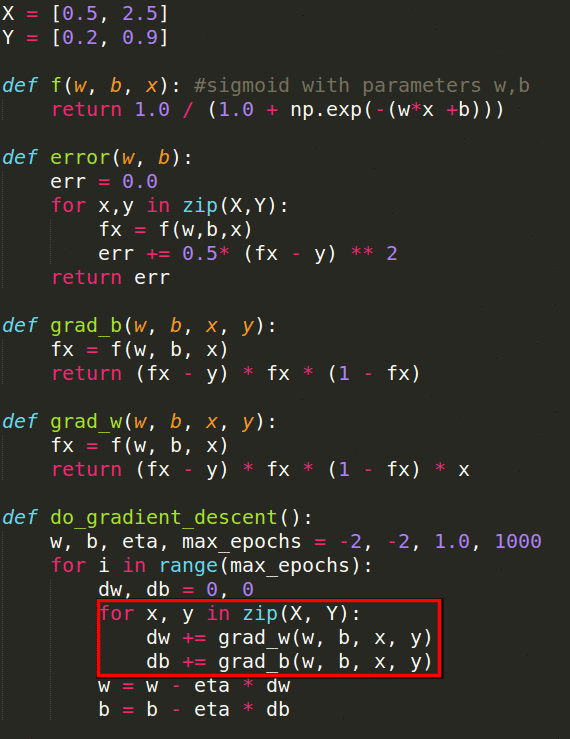
\includegraphics[scale=0.3]{images/module6/pseudo_code_sgd_crop_highlight.png}
			\end{figure}
		\end{overlayarea}
		
		\column{0.6\textwidth}
		\begin{overlayarea}{\textwidth}{\textheight}
			
			\begin{itemize}\justifying
				\item<2-> Notice that the algorithm goes over the entire data once before updating the parameters
				\item<3-> \only<3->{Why?} \onslide<4->{Because this is the true gradient of the loss as derived earlier (sum of the gradients of the losses corresponding to each data point)}
				
				\item<5-> \onslide<5->{No approximation.} \onslide<6->{Hence, theoretical guarantees hold (in other words each step guarantees that the loss will decrease)}
				\item<7-> What's the flipside? \onslide<8->{Imagine we have a million points in the training data.} \onslide<9->{To make 1 update to $w, b$ the algorithm makes a million calculations.} \onslide<10->{Obviously very slow!!}
				\item<11-> \only<11->{Can we do something better ?} \onslide<12->{Yes, let's look at stochastic gradient descent}
			\end{itemize}
			
			
		\end{overlayarea}
		
	\end{columns}
\end{frame}

\begin{frame}
	\begin{columns}
		\column{0.4\textwidth}
		\begin{overlayarea}{\textwidth}{\textheight}
			\vspace{-0.15in}
			\begin{figure}
				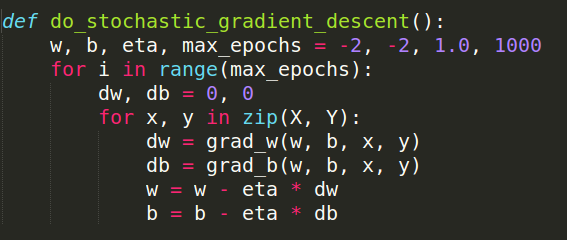
\includegraphics[scale=0.3]{images/module6/pseudo_code_stoch_gd_crop.png}
			\end{figure}
			
			\only<1-3>{
				\begin{figure}
					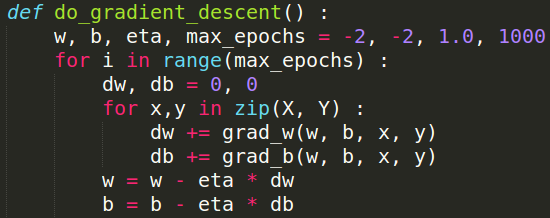
\includegraphics[scale=0.3]{images/module6/pseudo_code_sgd_crop_small.png}
				\end{figure}
			}
			
			\begin{itemize}\justifying 
				\item<6-> Stochastic because we are estimating the total gradient based on a single data point. \onslide<7->{Almost like tossing a coin only once and estimating P(heads).}
			\end{itemize} 
		\end{overlayarea}
		
		
		\column{0.6\textwidth}
		\begin{overlayarea}{\textwidth}{\textheight}
			
			\begin{itemize}\justifying
				\item<2-> Notice that the algorithm updates the parameters for every single data point
				\item<3-> Now if we have a million data points we will make a million updates in each epoch (1 epoch = 1 pass over the data; 1 step = 1 update)
				\item<4-> What is the flipside ? \onslide<5->{It is an approximate (rather stochastic) gradient}
				\item<8-> No guarantee that each step will decrease the loss
				\item<9-> Let's see this algorithm in action when we have a few data points
			\end{itemize}
			
		\end{overlayarea}
		
	\end{columns}
\end{frame}

\begin{frame}
	\begin{columns}
		\column{0.53\textwidth}
		\begin{overlayarea}{\textwidth}{\textheight}
			% \begin{itemize}\justifying
			% 	\item<37-> We see many oscillations. Why ? \onslide<38->{ Because we are making greedy decisions.}
			% 	\item<39-> Each point is trying to push the parameters in a direction most favorable to it \onslide<40->{(without being aware of how this affects other points)}
			% 	\item<41-> A parameter update which is locally favorable to one point may harm other points \onslide<42->{(its almost as if the data points are competing with each other)}
			% 	%\item<7-> Indeed we see that there is no guarantee that each local greedy move reduces the global error
			% 	\item<43-> Can we reduce the oscillations by improving our stochastic estimates of the gradient \onslide<44->{(currently estimated from just 1 data point at a time)}
			% 	\item<45-> Yes, let's look at mini-batch gradient descent
			% \end{itemize}
		\end{overlayarea}
		
		\column{0.47\textwidth}
		\begin{overlayarea}{\textwidth}{\textheight}
			
			\begin{figure}[ht]
				%\foreach[count=\i, evaluate=\i as \x using int(\i+5)] \n in {1,...,45}
				%{
				\foreach \n in {0,...,30} {%
					\pgfmathtruncatemacro\result{int(round(\n * 5))}
					\begin{tikzpicture}
						\sbox0{%
						\includegraphics[scale=0.414]{images/module6/stoch_gd3/2d_path\result.png}%
						}%
						\only<\n>{\node[above right,inner sep=0pt] at (0,0)  {\usebox{0}}};%
						\only<\n>{\node[red,font=\small](w) at (0.5\wd0,0.23\ht0) {w}};%
						\only<\n>{\node[red,font=\small](b) at (0,0.67\ht0) {b}};%
						\only<\n>{\draw[->, line width=0.2mm](w)--(0.6\wd0,0.23\ht0)};%
						\only<\n>{\draw[->, line width=0.2mm](b)--(0,0.8\ht0)};%
					\end{tikzpicture}
				}%
				
			\end{figure}
		\end{overlayarea}
	\end{columns}
\end{frame}

\begin{frame}
	\begin{columns}
		\column{0.53\textwidth}
		\begin{overlayarea}{\textwidth}{\textheight}
			\begin{itemize}\justifying
				\item<7-> We see many oscillations. Why ? \onslide<8->{ Because we are making greedy decisions.}
				\item<9-> Each point is trying to push the parameters in a direction most favorable to it \onslide<10->{(without being aware of how this affects other points)}
				\item<11-> A parameter update which is locally favorable to one point may harm other points \onslide<12->{(its almost as if the data points are competing with each other)}
				%\item<7-> Indeed we see that there is no guarantee that each local greedy move reduces the global error
				\item<13-> Can we reduce the oscillations by improving our stochastic estimates of the gradient \onslide<14->{(currently estimated from just 1 data point at a time)}
				\item<15-> Yes, let's look at mini-batch gradient descent
			\end{itemize}
		\end{overlayarea}
		
		\column{0.47\textwidth}
		\begin{overlayarea}{\textwidth}{\textheight}
			
			\begin{figure}[ht]
				%\foreach[count=\i, evaluate=\i as \x using int(\i+5)] \n in {1,...,45}
				%{
				\foreach \n in {0,...,15} {%
					\pgfmathtruncatemacro\result{int(round((\n+30) * 5))}
					\begin{tikzpicture}
						\sbox0{%
						\includegraphics[scale=0.414]{images/module6/stoch_gd3/2d_path\result.png}%
						}%
						\only<\n>{\node[above right,inner sep=0pt] at (0,0)  {\usebox{0}}};%
						\only<\n>{\node[red,font=\small](w) at (0.5\wd0,0.23\ht0) {w}};%
						\only<\n>{\node[red,font=\small](b) at (0,0.67\ht0) {b}};%
						\only<\n>{\draw[->, line width=0.2mm](w)--(0.6\wd0,0.23\ht0)};%
						\only<\n>{\draw[->, line width=0.2mm](b)--(0,0.8\ht0)};%
					\end{tikzpicture}
				}%
				
			\end{figure}
		\end{overlayarea}
	\end{columns}
\end{frame}


\begin{frame}
	\begin{columns}
		\column{0.5\textwidth}
		\begin{overlayarea}{\textwidth}{\textheight}
			\vspace{-0.15in}
			\begin{figure}
				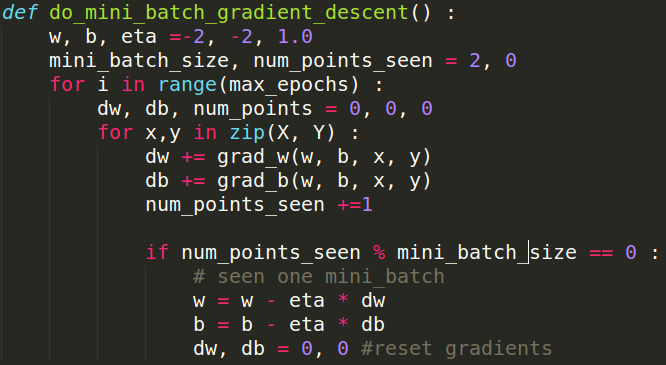
\includegraphics[scale=0.3]{images/module6/pseudo_code_mini_batch_gd_crop.png}
			\end{figure}
			
			\only<1-3>{
				\begin{figure}
					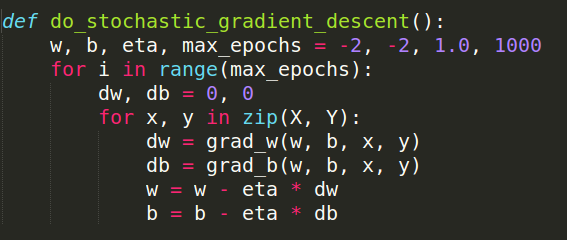
\includegraphics[scale=0.3]{images/module6/pseudo_code_stoch_gd_crop.png}
				\end{figure}
			}
		\end{overlayarea}
		
		
		\column{0.5\textwidth}
		\begin{overlayarea}{\textwidth}{\textheight}
			
			\begin{itemize}\justifying
				\item<1-> Notice that the algorithm updates the parameters after it sees $mini\_batch\_size$ number of data points
				\item<2-> The stochastic estimates are now slightly better
				\item<3-> Let's see this algorithm in action when we have k = 2
			\end{itemize}
			
		\end{overlayarea}
		
	\end{columns}
\end{frame}


\begin{frame}
	\begin{columns}
		\column{0.57\textwidth}
		\begin{overlayarea}{\textwidth}{\textheight}
			% \begin{itemize}\justifying
			% 	\item<39-> Even with a batch size of k=2 the oscillations have reduced slightly. \onslide<40->{Why ?} 
			% 	\item<41-> Because we now have slightly better estimates of the gradient \onslide<42->{[analogy: we are now tossing the coin k=2 times to estimate P(heads)]}
			% 	\item<43-> The higher the value of k the more accurate are the estimates 
			% 	\item<44-> In practice, typical values of k are 16, 32, 64
			% 	\item<45-> Of course, there are still oscillations and they will always be there as long as we are using an approximate gradient as opposed to the true gradient
			% \end{itemize}
		\end{overlayarea}
		
		\column{0.43\textwidth}
		\begin{overlayarea}{\textwidth}{\textheight}
			\begin{figure}
				\foreach \n in {0,...,25} {%
					\pgfmathtruncatemacro\result{int(round(\n * 2))}
					\begin{tikzpicture}
						\sbox0{\includegraphics[scale=0.38]{images/module6/mini_batch_gd5/2d_path\result.png}}% get width and height
						\only<\n>{\node[above right,inner sep=0pt] at (0,0)  {\usebox{0}}};
						\only<\n>{\node[red,font=\small](w) at (0.5\wd0,0.23\ht0) {w}};
						\only<\n>{\node[red,font=\small](b) at (0,0.67\ht0) {b}};
						\only<\n>{\draw[->, line width=0.2mm](w)--(0.6\wd0,0.23\ht0)};
						\only<\n>{\draw[->, line width=0.2mm](b)--(0,0.8\ht0)};
					\end{tikzpicture}
				}
			\end{figure}
		\end{overlayarea}
	\end{columns}
\end{frame}


\begin{frame}
	\begin{columns}
		\column{0.57\textwidth}
		\begin{overlayarea}{\textwidth}{\textheight}
			\begin{itemize}\justifying
				\item<9-> Even with a batch size of k=2 the oscillations have reduced slightly. \onslide<10->{Why ?} 
				\item<11-> Because we now have slightly better estimates of the gradient \onslide<12->{[analogy: we are now tossing the coin k=2 times to estimate P(heads)]}
				\item<13-> The higher the value of k the more accurate are the estimates 
				\item<14-> In practice, typical values of k are 16, 32, 64
				\item<15-> Of course, there are still oscillations and they will always be there as long as we are using an approximate gradient as opposed to the true gradient
			\end{itemize}
		\end{overlayarea}
		
		\column{0.43\textwidth}
		\begin{overlayarea}{\textwidth}{\textheight}
			\begin{figure}
				\foreach \n in {0,...,20} {%
					\pgfmathtruncatemacro\result{int(round((\n+25) * 2))}
					\begin{tikzpicture}
						\sbox0{\includegraphics[scale=0.38]{images/module6/mini_batch_gd5/2d_path\result.png}}% get width and height
						\only<\n>{\node[above right,inner sep=0pt] at (0,0)  {\usebox{0}}};
						\only<\n>{\node[red,font=\small](w) at (0.5\wd0,0.23\ht0) {w}};
						\only<\n>{\node[red,font=\small](b) at (0,0.67\ht0) {b}};
						\only<\n>{\draw[->, line width=0.2mm](w)--(0.6\wd0,0.23\ht0)};
						\only<\n>{\draw[->, line width=0.2mm](b)--(0,0.8\ht0)};
					\end{tikzpicture}
				}
			\end{figure}
		\end{overlayarea}
	\end{columns}
\end{frame}


\begin{frame}
	\begin{overlayarea}{\textwidth}{\textheight}
		\begin{block}{Some things to remember ....}
			\begin{itemize}\justifying
				\item 1 epoch = one pass over the entire data
				\item 1 step = one update of the parameters
				\item N = number of data points
				\item B = Mini batch size
				      
				      \begin{table}
				      	\begin{tabular}{cc}
				      		\hline\hline
				      		Algorithm                        & \# of steps in 1 epoch   \\
				      		\hline
				      		Vanilla (Batch) Gradient Descent & \only<2->{1}             \\
				      		Stochastic Gradient Descent      & \only<3->{N}             \\
				      		Mini-Batch Gradient Descent      & \only<4->{$\frac{N}{B}$} \\
				      		\hline\hline
				      	\end{tabular}
				      \end{table}
				      
			\end{itemize}
		\end{block}
	\end{overlayarea}
\end{frame}

\begin{frame}
	\fontsize{16pt}{7.2}\selectfont
	\textit{Similarly, we can have stochastic versions of Momentum based gradient descent and Nesterov accelerated based gradient descent}
\end{frame}


\begin{frame}
	\begin{columns}
		\column{0.5\textwidth}
		\begin{overlayarea}{\textwidth}{\textheight}
			\begin{figure}
				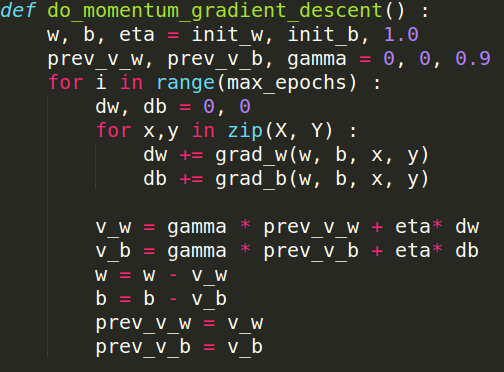
\includegraphics[scale=0.3]{images/module6/pseudo_code_mom_crop.png}
			\end{figure}
		\end{overlayarea}
		
		\column{0.5\textwidth}
		\begin{overlayarea}{\textwidth}{\textheight}
			\begin{figure}
				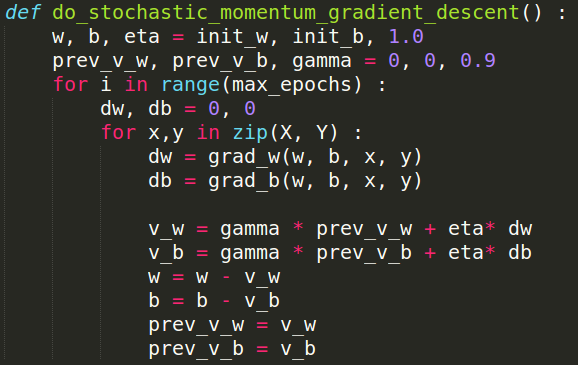
\includegraphics[scale=0.3]{images/module6/pseudo_code_stoch_mom_crop.png}
			\end{figure}
		\end{overlayarea}
	\end{columns}
\end{frame}

\begin{frame}
	\begin{columns}
		\column{0.5\textwidth}
		\begin{overlayarea}{\textwidth}{\textheight}
			\begin{figure}
				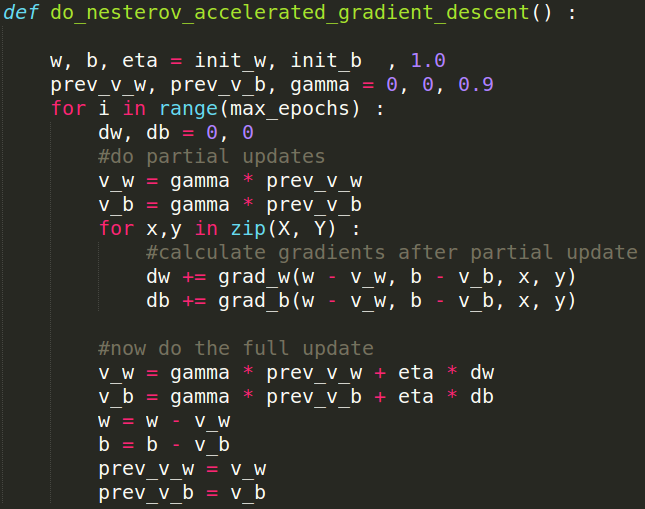
\includegraphics[scale=0.3]{images/module6/pseudo_code_nag_crop.png}
			\end{figure}
		\end{overlayarea}
		
		\column{0.5\textwidth}
		\begin{overlayarea}{\textwidth}{\textheight}
			\begin{figure}
				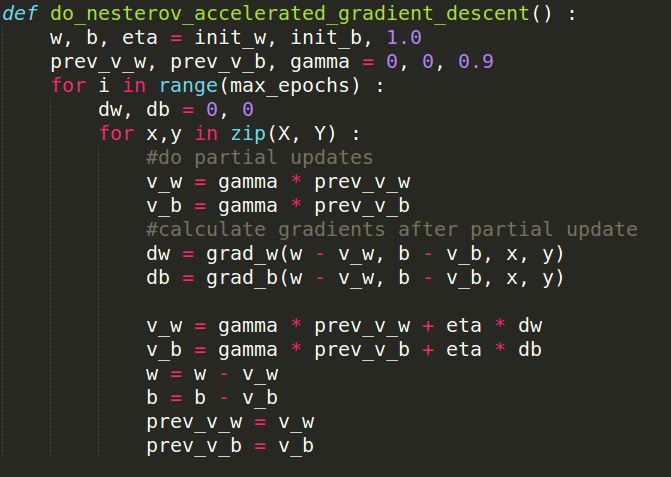
\includegraphics[scale=0.3]{images/module6/pseudo_code_stoch_nag_crop.png}
			\end{figure}
		\end{overlayarea}
	\end{columns}
\end{frame}



\begin{frame}
	\begin{columns}
		
		\column{0.6\textwidth}
		\begin{overlayarea}{\textwidth}{\textheight}
			
			\begin{itemize}\justifying 
				\item<2-> While the stochastic versions of both Momentum [blue] and NAG [red] exhibit oscillations the relative advantage of NAG over Momentum still holds \onslide<3->{(i.e., NAG takes relatively shorter u-turns)}
				\item<4-> Further both of them are faster than stochastic gradient descent \onslide<5->{(after 60 steps, stochastic gradient descent [black - top figure] still exhibits a very high error whereas NAG and Momentum are close to convergence)}
			\end{itemize} 
		\end{overlayarea}
		
		\column{0.4\textwidth}
		\begin{overlayarea}{\textwidth}{\textheight}
			\vspace{-0.1in}
			\begin{tikzpicture}
				\sbox0{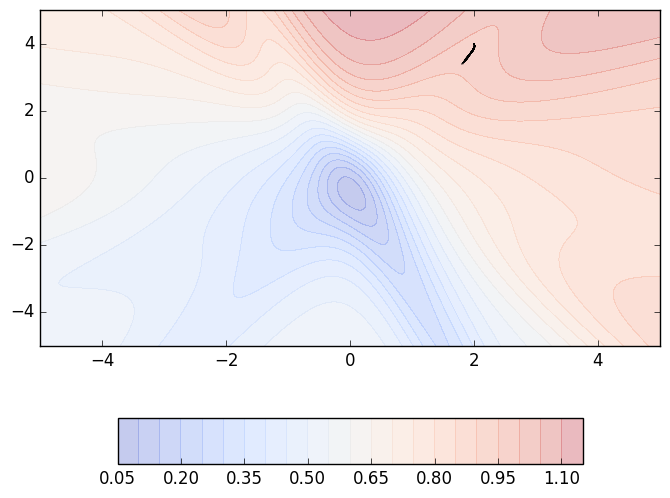
\includegraphics[scale=0.3]{images/module6/stoch_gd6/2d_path60.png}}% get width and height
				\node[above right,inner sep=0pt] at (0,0)  {\usebox{0}};
				\node[red](w) at (0.5\wd0,0.23\ht0) {w};
				\node[red](b) at (0,0.67\ht0) {b};
				\draw[->, line width=0.2mm](w)--(0.6\wd0,0.23\ht0);
				\draw[->, line width=0.2mm](b)--(0,0.8\ht0);
			\end{tikzpicture}
			
			\vspace{-0.05in}
			\begin{tikzpicture}
				\sbox0{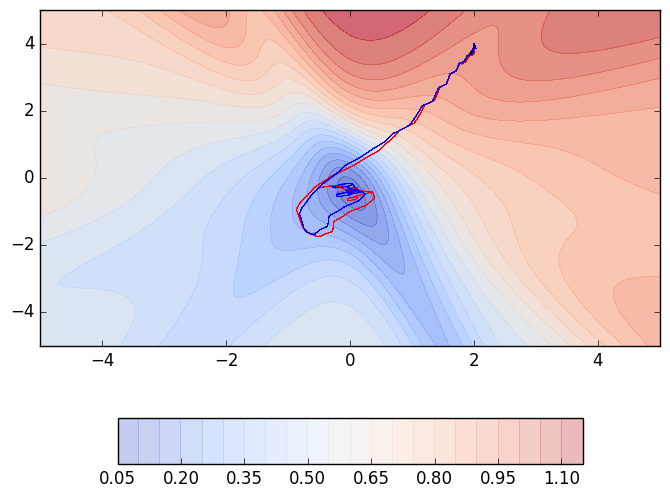
\includegraphics[scale=0.3]{images/module6/stoch_nag6/2d_path60.png}}% get width and height
				\node[above right,inner sep=0pt] at (0,0)  {\usebox{0}};
				\node[red](w) at (0.5\wd0,0.23\ht0) {w};
				\node[red](b) at (0,0.67\ht0) {b};
				\draw[->, line width=0.2mm](w)--(0.6\wd0,0.23\ht0);
				\draw[->, line width=0.2mm](b)--(0,0.8\ht0);
			\end{tikzpicture}
		\end{overlayarea}
		
	\end{columns}
\end{frame}

\begin{frame}
	\fontsize{16pt}{7.2}\selectfont
	\textit{And, of course, you can also have the mini batch version of Momentum and NAG...\onslide<2->{I leave that as an exercise :-)}}
\end{frame}
